\chapter{Systembeschreibung}
\label{system}

Das nachfolgende Kapitel befasst sich mit der Beschreibung der Technologien und Vorgehensweisen, die zur Link Discovery im Rahmen dieser Arbeit angewendet wurden. Dazu zählen im Einzelnen die gewählte Datenbank MongoDB, das Datenmodell des Zielgraphen und das daraus resultierende Vorgehen und die Architektur des Systems zur Link Discovery.

\section{MongoDB}
\label{mongo}

Zur Umsetzung der Link Discovery wurde das Datenbankmanagementsystem MongoDB \cite{mo2013} gewählt. Bei MongoDB handelt es sich um eine quelloffene dokumentenorientierte Datenbank.

Im Gegensatz zu traditionellen relationalen Datenbanksystemen verzichtet MongoDB dabei auf eine tabellenförmige Struktur der Daten und speichert Datensätze in Form von so genannten \emph{Dokumenten}. Dabei handelt es sich um hierarchische Schlüssel-/Wertpaare, die schemalos in so genannten \emph{Collections} gespeichert werden. Schemalos bedeutet dabei, dass die Dokumente innerhalb einer Collection nicht alle dieselbe Struktur besitzen müssen.

Zur Repräsentation der Dokumente verwendet MongoDB ein Format, dass sich sehr an JSON \cite{json2006} anlehnt. JSON ist ein menschenlesbares Datenaustauschformat, das aus der Objektnotation der Programmiersprache JavaScript abgeleitet wurde. Das Datenformat von MongoDB ist BSON \cite{bson2013}, eine binäre Repräsentation von JSON, die einige zusätzliche Datentypen unterstützt. 

Listing \ref{lst:json} zeigt ein Beispiel für ein Dokument in MongoDB. Das Feld \emph{\_id} ist hierbei ein  Bezeichner vom Typ \emph{ObjectID}. Dieser stellt einen global eindeutigen Bezeichner dar, der benutzt werden kann, um Dokumente zu referenzieren. Innerhalb einer Collection ist \emph{\_id} dabei grundsätzlich eindeutig. Das Feld \emph{address} zeigt, dass Dokumente weitere Dokumente enthalten können. Das Feld \emph{friends} zeigt, dass Werte für Schlüssel auch Arrays von Werten sein können. Diese sind dabei nicht auf primitive Typen wie Zeichenketten oder Zahlen beschränkt, sondern können auch weitere Dokumente sein.

\begin{lstlisting}[language=json, label={lst:json}, caption={Ein Beispiel für ein Dokument in MongoDB}]
{
    "_id" : ObjectId("51efc20147cae77dfc02e0ac"),
    "name" : "Bob",
    "age": 25,
    "address": {
        "city": "Leipzig",
        "street": "Karl-Liebknecht-Str. 132"
        "zip": "04277"
    },
    "friends" : [
        "alice",
        "fred",
        "jason"
    ]
}
\end{lstlisting}

MongoDB unterstützt Anfragen über ein Binärprotokoll, welches über so genannte \emph{Treiber} in vielen Programmiersprachen abstrahiert zur Verfügung steht. Dabei sind vielfältige Lese- und Schreiboperationen möglich, die komplexe Abfragen und Operationen auf den gespeicherten Daten zulassen. Außerdem bietet MongoDB eine Implementierung des MapReduce-Programmiermodells (siehe \ref{mapreduce}) sowie die Möglichkeit, Indizes auf allen Hierarchieebenen der Dokumente zu nutzen. Für interaktive Operationen steht die \emph{Mongo Shell} zur Verfügung, welche Abfragen mittels der Programmiersprache JavaScript erlaubt und somit einen Treiber für diese Sprache darstellt.

Aufgrund der genannten Eigenschaften stellt MongoDB einen exzellenten Ausgangspunkt für die Link Discovery im Rahmen dieser Arbeit dar. Durch die vorhandene Schemaflexibilität können die Daten in der gerade benötigten Form gespeichert und abgefragt werden. Durch die Unterstützung von MapReduce mit mehreren Rechnern lassen sich Berechnungen wie die der Kookkurrenz (siehe \ref{mapreduce_cooccurence}) parallelisieren und somit beschleunigen.

Aus diesen Gründen stellt MongoDB das zentrale technische Element für die Link Discovery im Rahmen dieser Arbeit dar. Sobald die Daten aus den externen und internen Quellen in MongoDB importiert wurden, können die folgenden Schritte direkt mit Datenbankabfragen realisiert werden.

\section{Datenmodell}

Nach der Auswahl eines geeigneten Datenbanksystems sollte das Datenmodell des Ergebnisses genauer spezifiziert werden. Ist dieses vor der Link Discovery klar, können die einzelnen benötigten Schritte zur Erreichung des Zieles einfacher definiert werden.

Generell handelt es sich bei dem gewünschten Ergebnis um einen gerichteten Multigraph. Dieser repräsentiert Objekte, oder auch \emph{Knoten}, zwischen denen paarweise Verbindungen, die \emph{Kanten} bestehen. Die Besonderheit eines Multigraphen ist dabei, dass zwischen zwei Knoten auch mehrere Kanten existieren dürfen \cite{rd2012}. Dies ist dem gewählten Lösungsansatz geschuldet, da zwischen Wörtern und Wortgruppen verschiedenartige Beziehungen existieren können.

Somit müssen für das Datenmodell die beiden Entitäten \emph{Knoten} und \emph{Kante} modelliert werden.
Das komplette Datenmodell des Graphen nach der Integration aller Datenquellen ist in Anhang \ref{complete_data_model} dargestellt.

\subsection{Knoten}

Die Knoten repräsentierendie Wörter und Wortgruppen zwischen denen durch Link Discovery Verbindungen hergestellt werden sollen. Sie enthalten als benötigte Attribute eine Zeichenkette und ein Attribut Sprache. Die Kombination dieser beiden Attribute ist innerhalb der Knotenmenge eindeutig. Außerdem erhält jeder Knoten zur einfacheren Referenzierung einen eindeutigen Bezeichner.

Neben diesen immer vorhandenen Attributen kann ein Knoten beliebig viele weitere Eigenschaften besitzen. Diese Eigenschaften dienen dazu, den Begriffen, die die Knoten existieren, für spätere Verwendungen zusätzlichen Kontext zu geben. Im Wesentlichen definieren sich diese zusätzlichen Eigenschaften aus den Datenquellen, die zum Zweck der Link Discovery in den Graph integriert werden.

Zur besseren Kapselung und Übersicht sollten die zusätzlichen Eigenschaften in weitere Entitäten gekapselt werden. Die Struktur dieser zusätzlichen Typen kann dann zum Zeitpunkt der Integration der jeweiligen Datenquelle definiert werden.

Das resultierende Knotenmodell ist in Abbildung \ref{fig:node_erd} dargestellt.

\begin{figure}
\centering
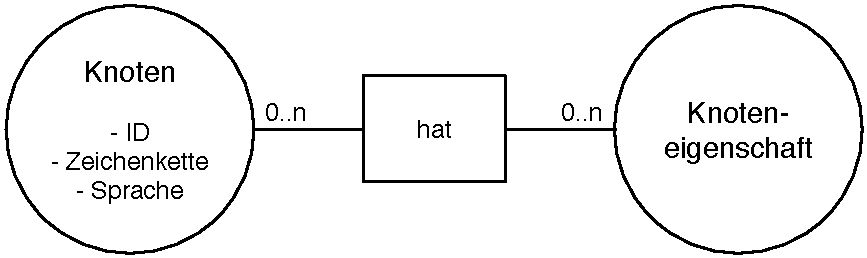
\includegraphics[width=0.6\textwidth]{node_erd}
\caption{Knotenmodell als Entity-Relationship-Diagramm}
\label{fig:node_erd}
\end{figure}

\subsection{Kanten}

Eine Kante ist im Wesentlichen durch die Knoten, die sie verbindet, beschrieben. Sie stellt einen irgendwie gearteten Zusammenhang zwischen zwei Knoten dar. Sie ist dabei gerichtet, um auch assymetrische Zusammenhänge zwischen Knoten abbilden zu können.

Somit sind die einzig immer benötigten Attribute der Quell- und Zielknoten und der Typ der Kante. Zusätzlich erhält jede Kante einen eindeutigen Bezeichner.

Alle weiteren Eigenschaften der Kante hängen vom Typ ab. Dies können beispielsweise Maße sein, die ein Kantengewicht darstellen. Da eine Kante nur genau einen Typ haben kann, werden die zusätzlichen Kanteneigenschaften einfach als Attribute an der Kante annotiert.

Das beschriebene Kantenmodell ist in Abbildung \ref{fig:edge_erd} dargestellt.

\begin{figure}
\centering
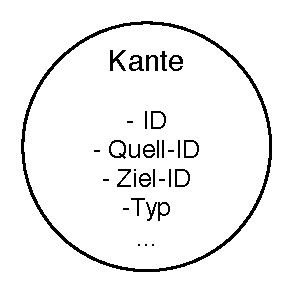
\includegraphics[width=0.2\textwidth]{edge_erd}
\caption{Kantenmodell als Entity-Relationship-Diagramm}
\label{fig:edge_erd}
\end{figure}

\subsection{Technische Umsetzung}

Um das beschriebene Datenmodell in MongoDB umzusetzen, muss es in eine Dokumentenform überführt werden. Dazu bietet sich an, Knoten in Kanten in unterschiedlichen Collections zu speichern, um sie voneinander zu trennen.

Somit stellt sich anschließend die Frage, wie die Knoten und Kanten als Dokumente repräsentiert werden. Durch die durch MongoDB gegebene Schemaflexibilität lassen sich die optionalen Eigenschaften von Knoten und Kanten direkt in den Dokumenten speichern.

Im Fall der Knoten bietet sich daher an, die zusätzlichen Eigenschaften als Unterdokumente des Knotens zu behandeln. Der Schlüssel für diese Unterdokumente ist dabei der Name der zusätzlichen Eigenschaft. Dadurch lassen sich die Knoten gut filtern, da die Abfrage auf das Vorhandensein des jeweiligen Schlüssels angepasst sein kann. Listing \ref{lst:node_json} zeigt ein Beispiel für einen Knoten in JSON-Notation. Arrays mit vielen Elementen sind dabei verkürzt dargestellt.

Die Kanten können direkt als Dokumente abgebildet werden. Über den Typ ergeben sich zusätzliche Eigenschaften. Listing \ref{lst:edge_json} zeigt beispielhaft ein Kantendokument für eine Tag-Kookkurrenz in JSON-Notation.

\begin{lstlisting}[language=json, label={lst:node_json}, caption={Knotendokument in JSON}]
{
    "_id" : ObjectId("51efc22447cae77dfc03e16b"),
    "language" : "de",
    "string" : "segeln",
    "languageDetection" : {
        "language" : "de",
        "confidence" : 1
    },
    "tagProperties" : {
        "occurenceCount" : 4678,
        "articleCount" : 2347,
        "designCount" : 2331,
        "articleIDs" : [ 
            4961057, 
            4977725, 
            ...
        ],
        "designIDs" : [ 
            1645572, 
            2216059, 
            ...
        ]
    },
    "wortschatzProperties" : {
        "synonyms" : [ 
            "flattern", 
            "fliegen", 
            "gaukeln", 
            ...
        ]
    }
}
\end{lstlisting}

\begin{lstlisting}[language=json, label={lst:edge_json}, caption={Kantendokument in JSON}]
{
        "_id" : ObjectId("51efd6f61177ff360605bd99"),
        "source" : ObjectId("51efc1af47cae77dfc00c3f8"),
        "target" : ObjectId("51efc1e047cae77dfc02087c"),
        "type" : "tag-co-occurence",
        "occurences" : 1,
        "dice" : 0.0001317089232795522,
        "jaccard" : 0.00006585879873551106,
        "cosine" : 0.008115343414514944
}
\end{lstlisting}

Nachdem die Datenformate definiert sind, beschäftigt sich das folgende Kapitel mit der Architektur des implementierten Link Discovery-Systems.

\section{Systemarchitektur}

Nach erfolgter Technologieauswahl und Modellierung der Daten soll im nächsten Abschnitt die Umsetzung der Link Discovery beschrieben werden.

Da die Mongo Shell eine vollwertige JavaScript-Laufzeitumgebung enthält und skriptbar ist, wurden die meisten Operationen im Rahmen dieser Arbeit als Skripte für diese Shell implementiert. Einzig der Import der Tag- und Clicktrackingdaten wurde mit Ruby-Skripten realisiert.

Die Schritte zur Link Discovery sind im Wesentlichen für jede zu integrierende Datenquelle gleich. Sie umfassen den Import, die Bereinigung, die Reduktion, die Transformation und die Integration der Daten \cite{hkp2012}.

\begin{figure}
\centering
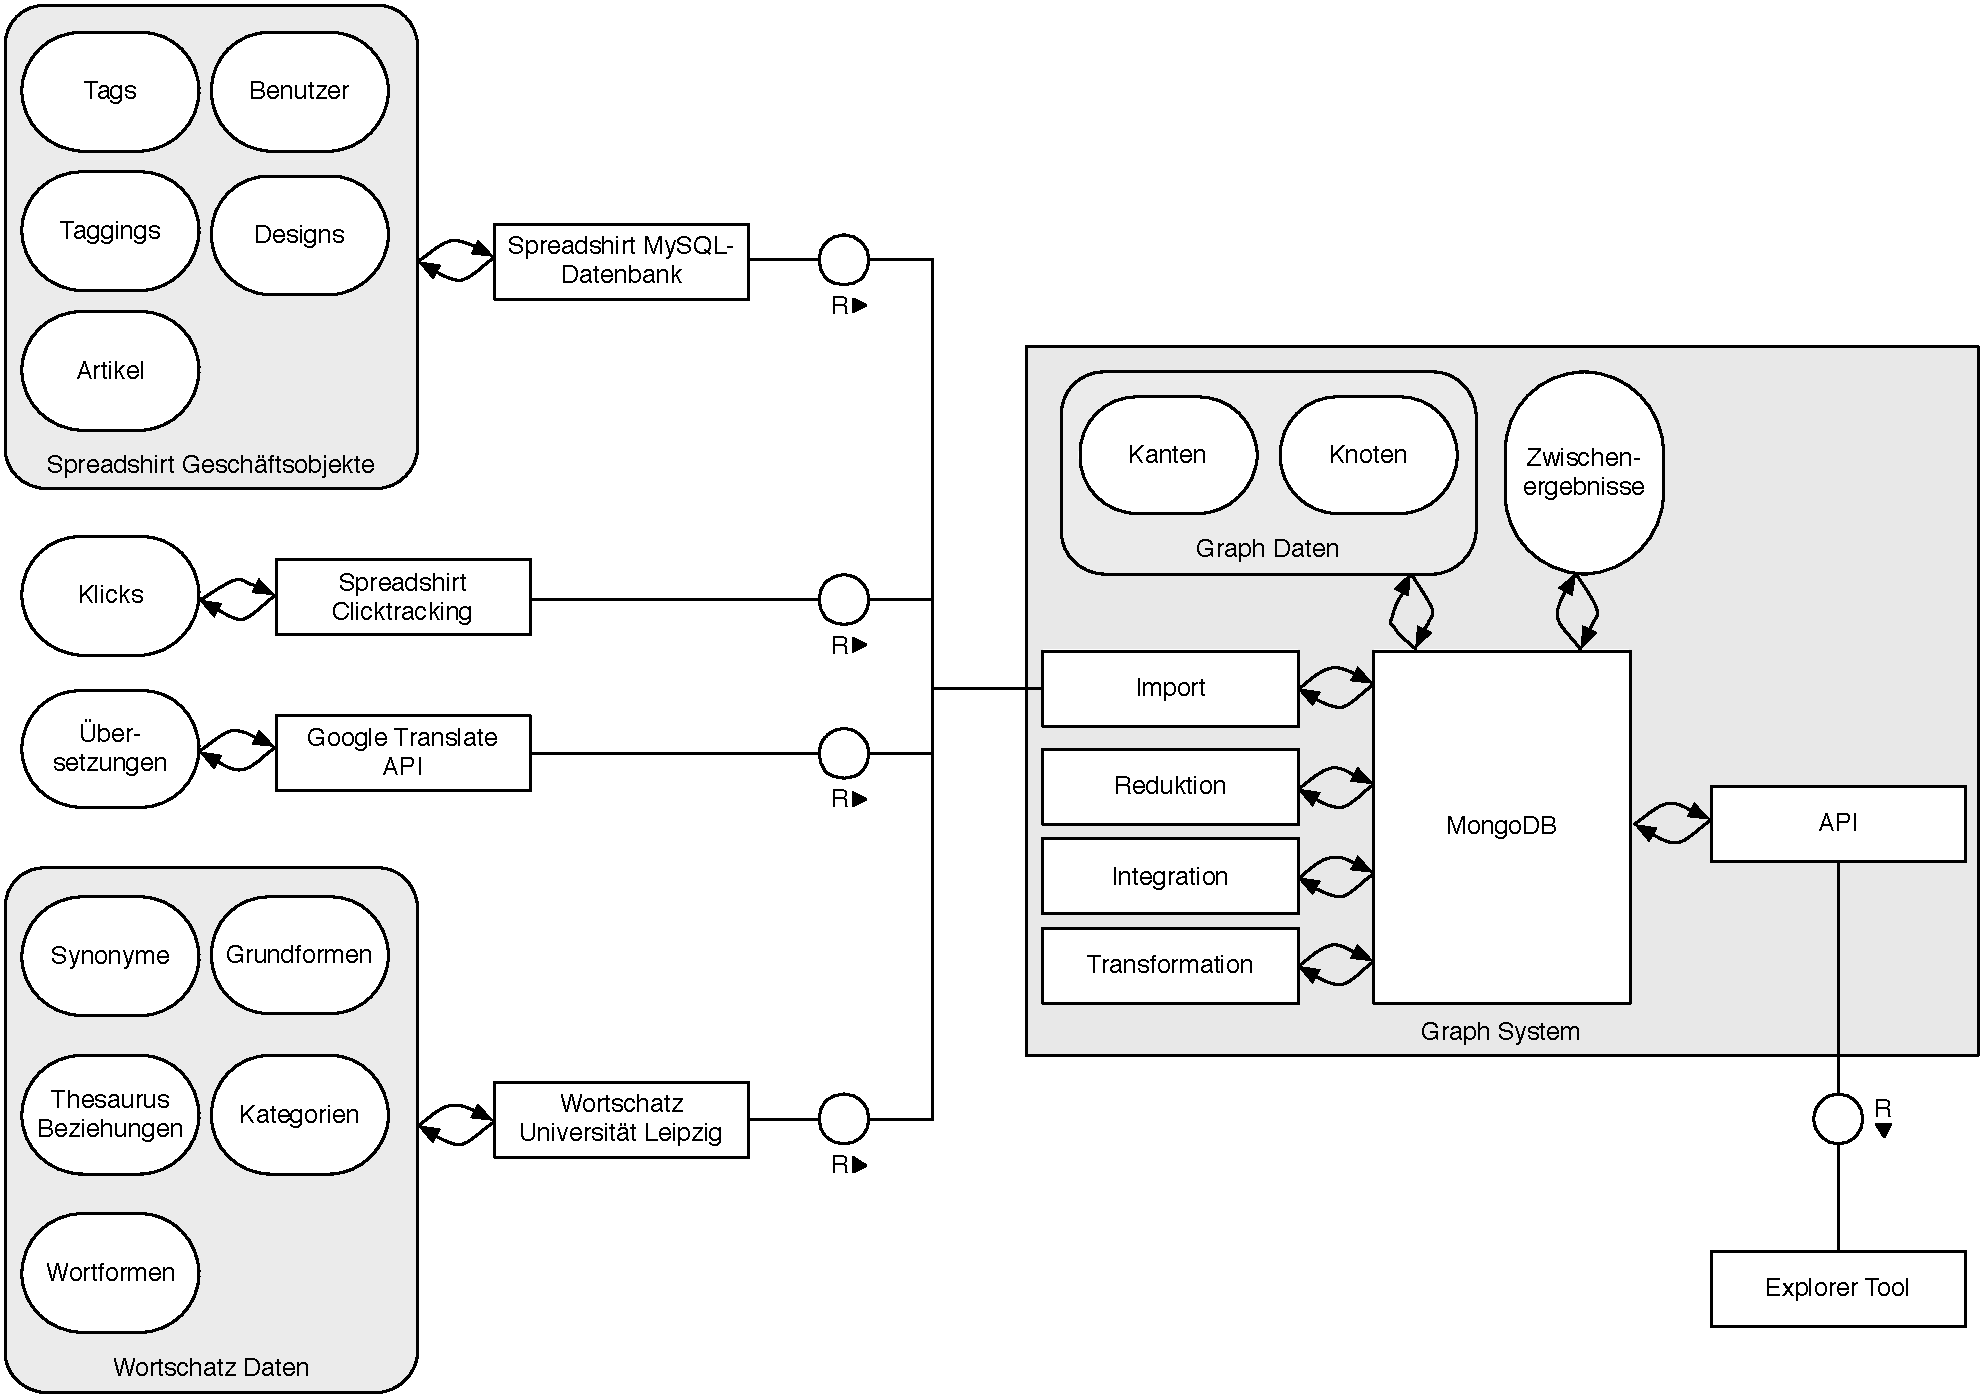
\includegraphics[width=1\textwidth]{architecture}
\caption{Systemarchitektur}
\label{fig:architecture}
\end{figure}

Abbildung \ref{fig:architecture} zeigt die komplette Architektur des implementierten Link Discovery Systems. Darin sind alle genutzten Datenquellen und die Daten, die sie bereit stellen, aufgeführt.

Für jede Datenquelle exisitiert ein Importskript, welches die Rohdaten importiert und in MongoDB speichert. Bei relationalen Datenquellen wie der Spreadshirt MySQL-Datenbank für die Tag-Daten wird pro Tabelle eine Collection und pro Zeile ein Dokument angelegt. Können nicht alle Daten importiert werden, wie beispielsweise bei der Wortschatz-API, kann das Importskript auch aufgrund der bisher im Graph vorhandenen Daten eine Auswahl an Anfragen an die externe Datenquelle erzeugen.

Im nachfolgenden Bereinigungsschritt werden die Daten so gut wie möglich von den in Abschnitt \ref{quality} beschriebenen Defekten befreit. Dazu zählen beispielsweise das Entfernen nicht nutzbarer Zeichen oder unvollständigen Datensätzen.

Der Reduktionsschritt dient zur Verkleinerung der Datenmenge. Dazu gehören beispielsweise Schritte zur Duplikatentfernung oder zur Auswahl relevanter Datensätze. In dieser Arbeit bestand die Haupteinschränkung der Datenmenge darin, nach Möglichkeit nur deutschsprachige Datensätze auszuwählen.

Der Schritt der Transformation überführt die Daten schließlich in eine Graphenform. Dies kann entweder über Kookkurrenz oder über eine andere, für die Art der importierten Daten geeignete, Methode erfolgen.

Das Integrationsskript für jede Datenquelle ist letztendlich für die Integration der Daten in den Zielgraphen verantwortlich. Dabei werden neue Informationen an die Knoten angefügt oder neue Kanten in den Graph integriert. In diesem Schritt passiert die Auflösung von eventuell vorhandenen temporären Bezeichnern in die entsprechenden im Graph vorhandenen eindeutigen Bezeichner.

Für die Abfrage der im Graph gespeicherten Informationen existiert außerdem eine API, welche Informationen zu Knoten und deren Nachbarn per HTTP als JSON-Dokumente zur Verfügung stellt. Diese API kann für die Einbindung der erzeugten Informationen in andere Applikationen genutzt werden. Über Anfrageparameter kann dabei die Gewichtung der einzelnen Kantentypen beeinflusst werden.

Eine Beispielanwendung, die die API des Link Discovery-Systems nutzt, ist der \emph{Tag Explorer}. Dabei handelt es sich um eine Browseranwendung, die die im Graph gespeicherten Beziehungen visualisiert und interaktiv erforschbar macht. Der Benutzer dieser Anwendung kann mit selbst gewählten Gewichtungen der Kanten den Graph durchsuchen. Außerdem werden, wenn vorhanden, über eine Anbindung der Spreadshirt-API zu der Zeichenkette des ausgewählten Knotens gefundene Designs angezeigt. In Abbildung \ref{fig:tag_explorer} ist ein Screenshot dieses Werkzeuges zu sehen.

\begin{figure}
\centering
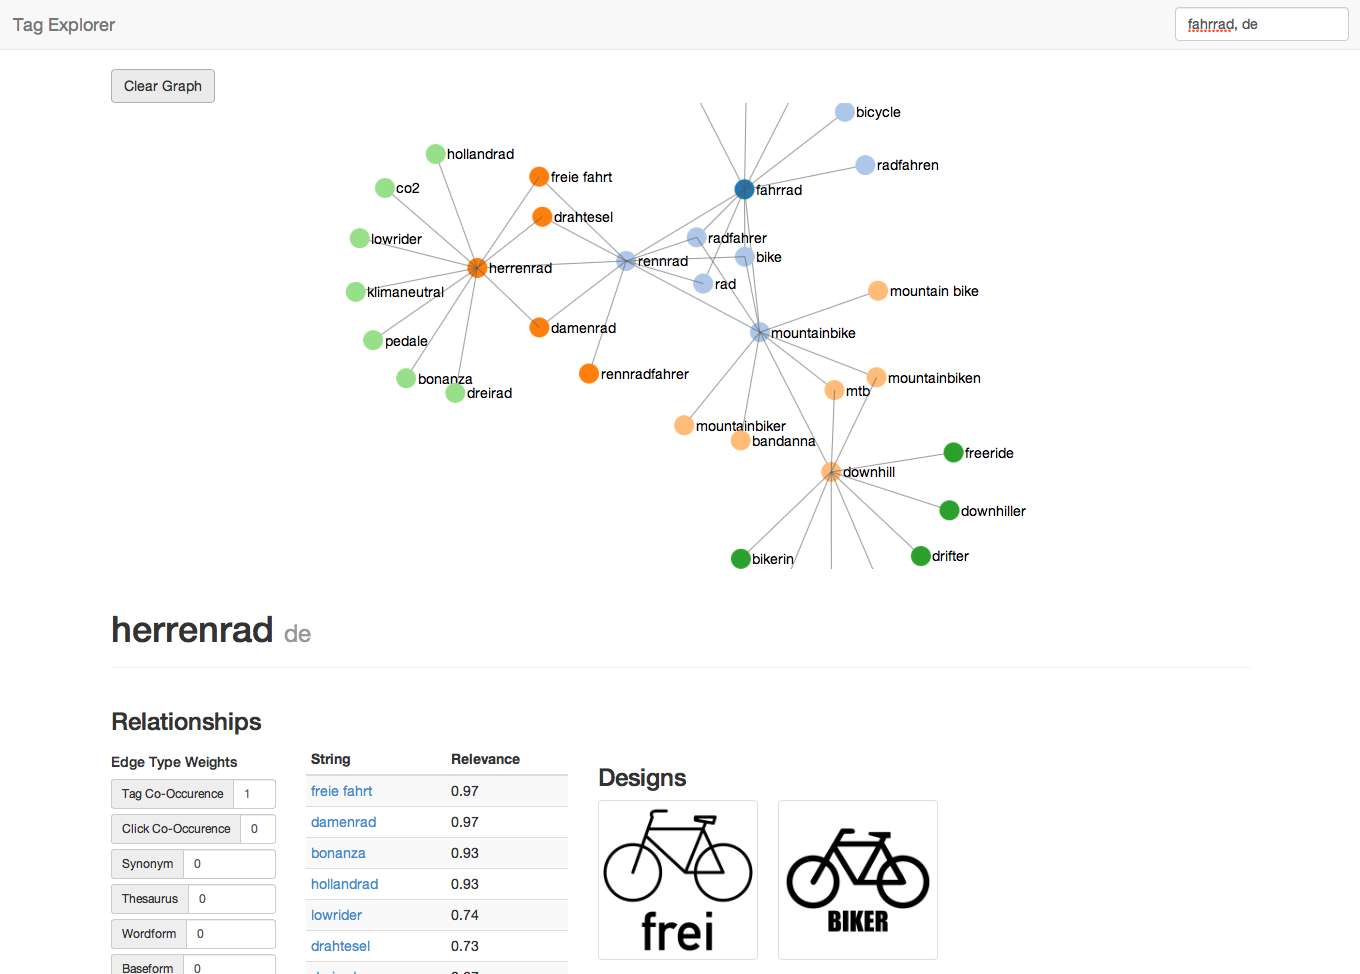
\includegraphics[width=0.9\textwidth]{tag_explorer}
\caption{Tag Explorer}
\label{fig:tag_explorer}
\end{figure}

Nachdem das System zur Link Discovery in diesem Kapitel beschrieben wurde, wird im nächsten Kapitel die praktische Durchführung und die Ergebnisse detailliert beschrieben.